\documentclass[letterpaper,12pt,fleqn]{article}
\usepackage{matharticle}
\pagestyle{empty}
\renewcommand{\o}{\theta}
\newcommand{\p}{\phi}
\newcommand{\G}{\Gamma}
\newcommand{\z}{\zeta}
\newcommand{\s}{\sigma}
\begin{document}
\section*{Conformal Mapping}

\begin{minipage}{3in}
  \begin{tikzpicture}
    \draw [<->] (-3,0) -- (3,0) node [right] {$x$};
    \draw [<->] (0,-3) -- (0,3) node [above] {$y$};
    \draw (0,0) arc (270:360:2);
    \draw [dashed] (1,0) -- (2.6,2);
    \draw [fill=black] (1.55,0.71) circle [radius=0.05];
    \node [above right] at (1.25,0) {$\o$};
  \end{tikzpicture}
\end{minipage}
\begin{minipage}{3in}
  $z(t)=x(t)+iy(t)$
  
  $z'(t)=x'(t)+iy'(t)$

  $\tan{\o}=\frac{dy}{dx}=\frac{y'(t)}{x'(t)}$

  $\o=\arg{z'(t)}$
\end{minipage}

\begin{definition}
  To say that a curve $C$ represented by $z(t)=x(t)+iy(t)$ is
  \emph{continuously differentiable} in an interval $[a,b]$ means that $z'(t)$
  exists and is continuous $\forall\,t\in[a,b]$.

  To say that $C$ is a \emph{regular curve} means that:
  \begin{enumerate}
  \item $C$ is continuously differentiable
  \item $z'(t)\ne0$, except at perhaps the endpoints
  \end{enumerate}
\end{definition}

\begin{theorem}
  Let $f(z)=u+iv$ be analytic in a domain $D$. The Jacobian of $f(z)$ is
  given by:
  \[J=\abs{f'(z)}^2\]
\end{theorem}

\begin{theproof}
  $J=\frac{\partial(u,v)}{\partial(x,y)}=
  \begin{vmatrix}
    u_x & u_y \\
    v_x & v_y \\
  \end{vmatrix}=u_xv_y-v_xu_y=u_xu_x=v_x(-v_x)=u_x^2+v_x^2$

  $f'(z)=f_x=u_x+iv_x$ \\
  $\abs{f'(z)}=\sqrt{u_x^2+v_x^2}$ \\
  $\abs{f'(z)}^2=u_x^2+v_x^2$

  $J=\abs{f'(z)}^2$
\end{theproof}

\begin{definition}
  To say that the mapping $u=u(x,y)$ and $v=v(x,y)$ defined on a domain $D$ is
  \emph{conformal} in $D$ means that the angle between any two intersecting
  regular curves in $z$ is preserved in $w$ under the map.
\end{definition}

\begin{minipage}{2in}
  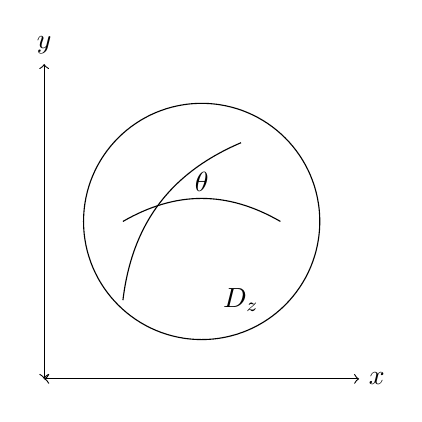
\begin{tikzpicture}
    \draw [<->] (0,0) -- (4,0) node [right] {$x$};
    \draw [<->] (0,0) -- (0,4) node [above] {$y$};
    \draw (2,2) circle [radius=1.5];
    \node at (2.5,1) {$D_z$};
    \draw (1,1) to [bend left=30] (2.5,3);
    \draw (1,2) to [bend left=30] (3,2);
    \node at (2,2.5) {$\o$};
  \end{tikzpicture}
\end{minipage}
\begin{minipage}{1.5in}
  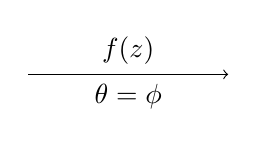
\begin{tikzpicture}
    \draw [->] (0,0) -- node [above] {$f(z)$} node [below] {$\o=\p$} (1in,0);
  \end{tikzpicture}
\end{minipage}
\begin{minipage}{2in}
  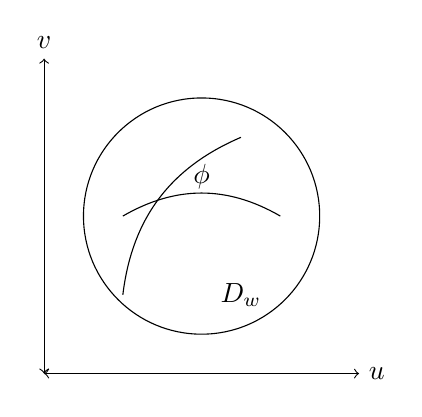
\begin{tikzpicture}
    \draw [<->] (0,0) -- (4,0) node [right] {$u$};
    \draw [<->] (0,0) -- (0,4) node [above] {$v$};
    \draw (2,2) circle [radius=1.5];
    \node at (2.5,1) {$D_w$};
    \draw (1,1) to [bend left=30] (2.5,3);
    \draw (1,2) to [bend left=30] (3,2);
    \node at (2,2.5) {$\p$};
  \end{tikzpicture}
\end{minipage}

\begin{theorem}
  Let $f(z)=u(x,y)+iv(x,y)$ be a continuously differentiable mapping on a
  domain $D$ such that $J\ne0$ in $D$:
  \[f(z)\ \mbox{is analytic in}\ D\iff\mbox{the mapping is conformal on}\ D\]
\end{theorem}

\begin{theproof}
  \listbreak
  \begin{description}
  \item $\implies$ Assume $f(z)$ is analytic in $D$

    Let $C_1: p_1(t)$ and $C_2: p_2(t)$ be two regular curves in $D$ on
    $[a,b]$ intersecting at $z_0\in D$ \\
    $z_0=p_1(t_0)=p_2(t_0)$ for some $t_0\in[a,b]$ \\
    Let $\o$ be the angle between $C_1$ and $C_2$ at $z_0$ \\
    $\o=\arg{\frac{{p_1}'(t_0)}{{p_2}'(t_0)}}=
    \arg{{p_2}'(t_0)}-\arg{{p_1}'(t_0)}$

    Let $\G_1: P_1(t)=f(p_1(t))$ and $\G_2: P_2(t)=f(p_2(t))$ be the
    corresponding image curves \\
    $\G_1$ and $\G_2$ intersect at $w_0=f(z_0)$ \\
    Let $\p$ be the angle between $\G_1$ and $\G_2$ at $w_0$
    \begin{eqnarray*}
      \p &=& \arg{\frac{{P_1}'(t_0)}{{P_2}'(t_0)}} \\
      &=& \arg{{P_1}'(t_0)}-\arg{{P_2}'(t_0)} \\
      &=& \arg[f'(p_1(t_0)){p_1}'(t_0)]-\arg[f'(p_2(t_0)){p_2}'(t_0)] \\
      &=& \arg[f'(z_0){p_1}'(t_0)]-\arg[f'(z_0){p_2}'(t_0)] \\
      &=& \arg{f'(z_0)}+\arg{{p_1}'(t_0)}-\arg{f'(z_0)}-\arg{{p_2}'(t_0)} \\
      &=& \arg{{p_1}'(t_0)}-\arg{{p_2}'(t_0)} \\
      &=& \o
    \end{eqnarray*}
    
  \item $\impliedby$ Assume that the mapping is conformal
    
  \end{description}
\end{theproof}
\newpage
\begin{example}
  Let $D$ be $\abs{z-1}<1$ and $f(z)=z^3$

  $f(z)$ is entire, so it is analytic in $D$

  $f'(z)=3z^2$ \\
  $f'(z)=0$ at $z=0\notin D$ \\
  $f'(z)\ne 0$ in $D$

  $\therefore f(z)$ is conformal in $D$
\end{example}

\begin{example}
  Let $D$ be $\abs{\z}<1$ and $z=w(\z)=(1+\z)^2$

  $w(\z)$ is entire, so it is analytic in $D$

  $w'(\z)=2(1+\z)$ \\
  $w'(\z)=0$ at $z=-1\notin D$ \\
  $w'(\z)\ne 0$ in $D$

  $\therefore w(\z)$ is conformal in $D$

  But what does the image look like?

  \begin{minipage}{3in}
    \begin{tikzpicture}
      \draw [<->] (-3,0) -- (3,0);
      \draw [<->] (0,-3) -- (0,3);
      \draw [->] (3,2) -- node [above] {$f(z)$} (4.5,2);
      \draw (0,0) circle [radius=2];
      \draw [fill=black] ({sqrt(2)},{-sqrt(2)}) circle [radius=0.05];
      \node [below right] at ({sqrt(2)},{-sqrt(2)}) {$\s=e^{i\o}$};
    \end{tikzpicture}
  \end{minipage}
  \begin{minipage}{3in}
    \begin{tikzpicture}
      \draw [<->] (-1,0) -- (5,0);
      \draw [<->] (0,-3) -- (0,3);
      \draw [domain=0:360,smooth] plot (canvas polar cs:angle=\x,
      radius={2cm*(1+cos(\x))});
      \node [below right] at (4,0) {$4$};
      \node [left] at (0,2) {$2$};
      \node [left] at (0,-2) {$-2$};
    \end{tikzpicture}
  \end{minipage}
  \begin{eqnarray*}
    z &=& (1+\s)^2 \\
    &=& (1+e^{i\o})^2 \\
    &=& (1+\cos{\o}+i\sin{\o})^2 \\
    &=& \left[2\cos^2\left(\frac{\o}{2}\right)+
      i2\sin\left(\frac{\o}{2}\right)\cos\left(\frac{\o}{2}\right)\right]^2 \\
    &=& 4\cos^2\left(\frac{\o}{2}\right)\left[\cos\left(\frac{\o}{2}\right)+
      i\sin\left(\frac{\o}{2}\right)\right] \\
    &=& 4\cos^2\left(\frac{\o}{2}\right)e^{i\o}
  \end{eqnarray*}
  Now, let $z=re^{i\p}$ and let $\o=\p$:
  \begin{eqnarray*}
    re^{i\p} &=& 4\cos^2\left(\frac{\o}{2}\right)e^{i\o} \\
    r &=& 4\cos^2\left(\frac{\o}{2}\right) \\
    r &=& 2(1+\cos{\p})
  \end{eqnarray*}

  Which is a cardiod.
\end{example}
  
\end{document}
